\chapter{Теоретический раздел}

\section{Используемые распределения}

В качестве распределения генератора используется равномерное распределение. В качестве распределения обслуживающего аппарата используется распределение Эрланга.

\subsection{Равномерное распределение}
    
Говорят, что случайная величина X имеет равномерное распределение на отрезке $[a,b]$, если её функция плотности имеет вид:

\begin{equation*}
    f_X (x) =
    \begin{cases}
        \frac{1}{b-a}, x \in [a,b] \\
        0, x \notin [a, b] \\
    \end{cases}
\end{equation*}

Значения случайной величины с двух сторон ограничены и в границах интервала имеют одинаковую вероятность. В данном интервале плотность вероятности постоянна.

Функция распределения:

\begin{equation*}
F_X (x) =
    \begin{cases}
        0, x < a \\
        \frac{x - a}{b - a}, a \le x < b \\
        1, x \geq b \\
    \end{cases}
\end{equation*}

\begin{figure}[H]
    \begin{center}
    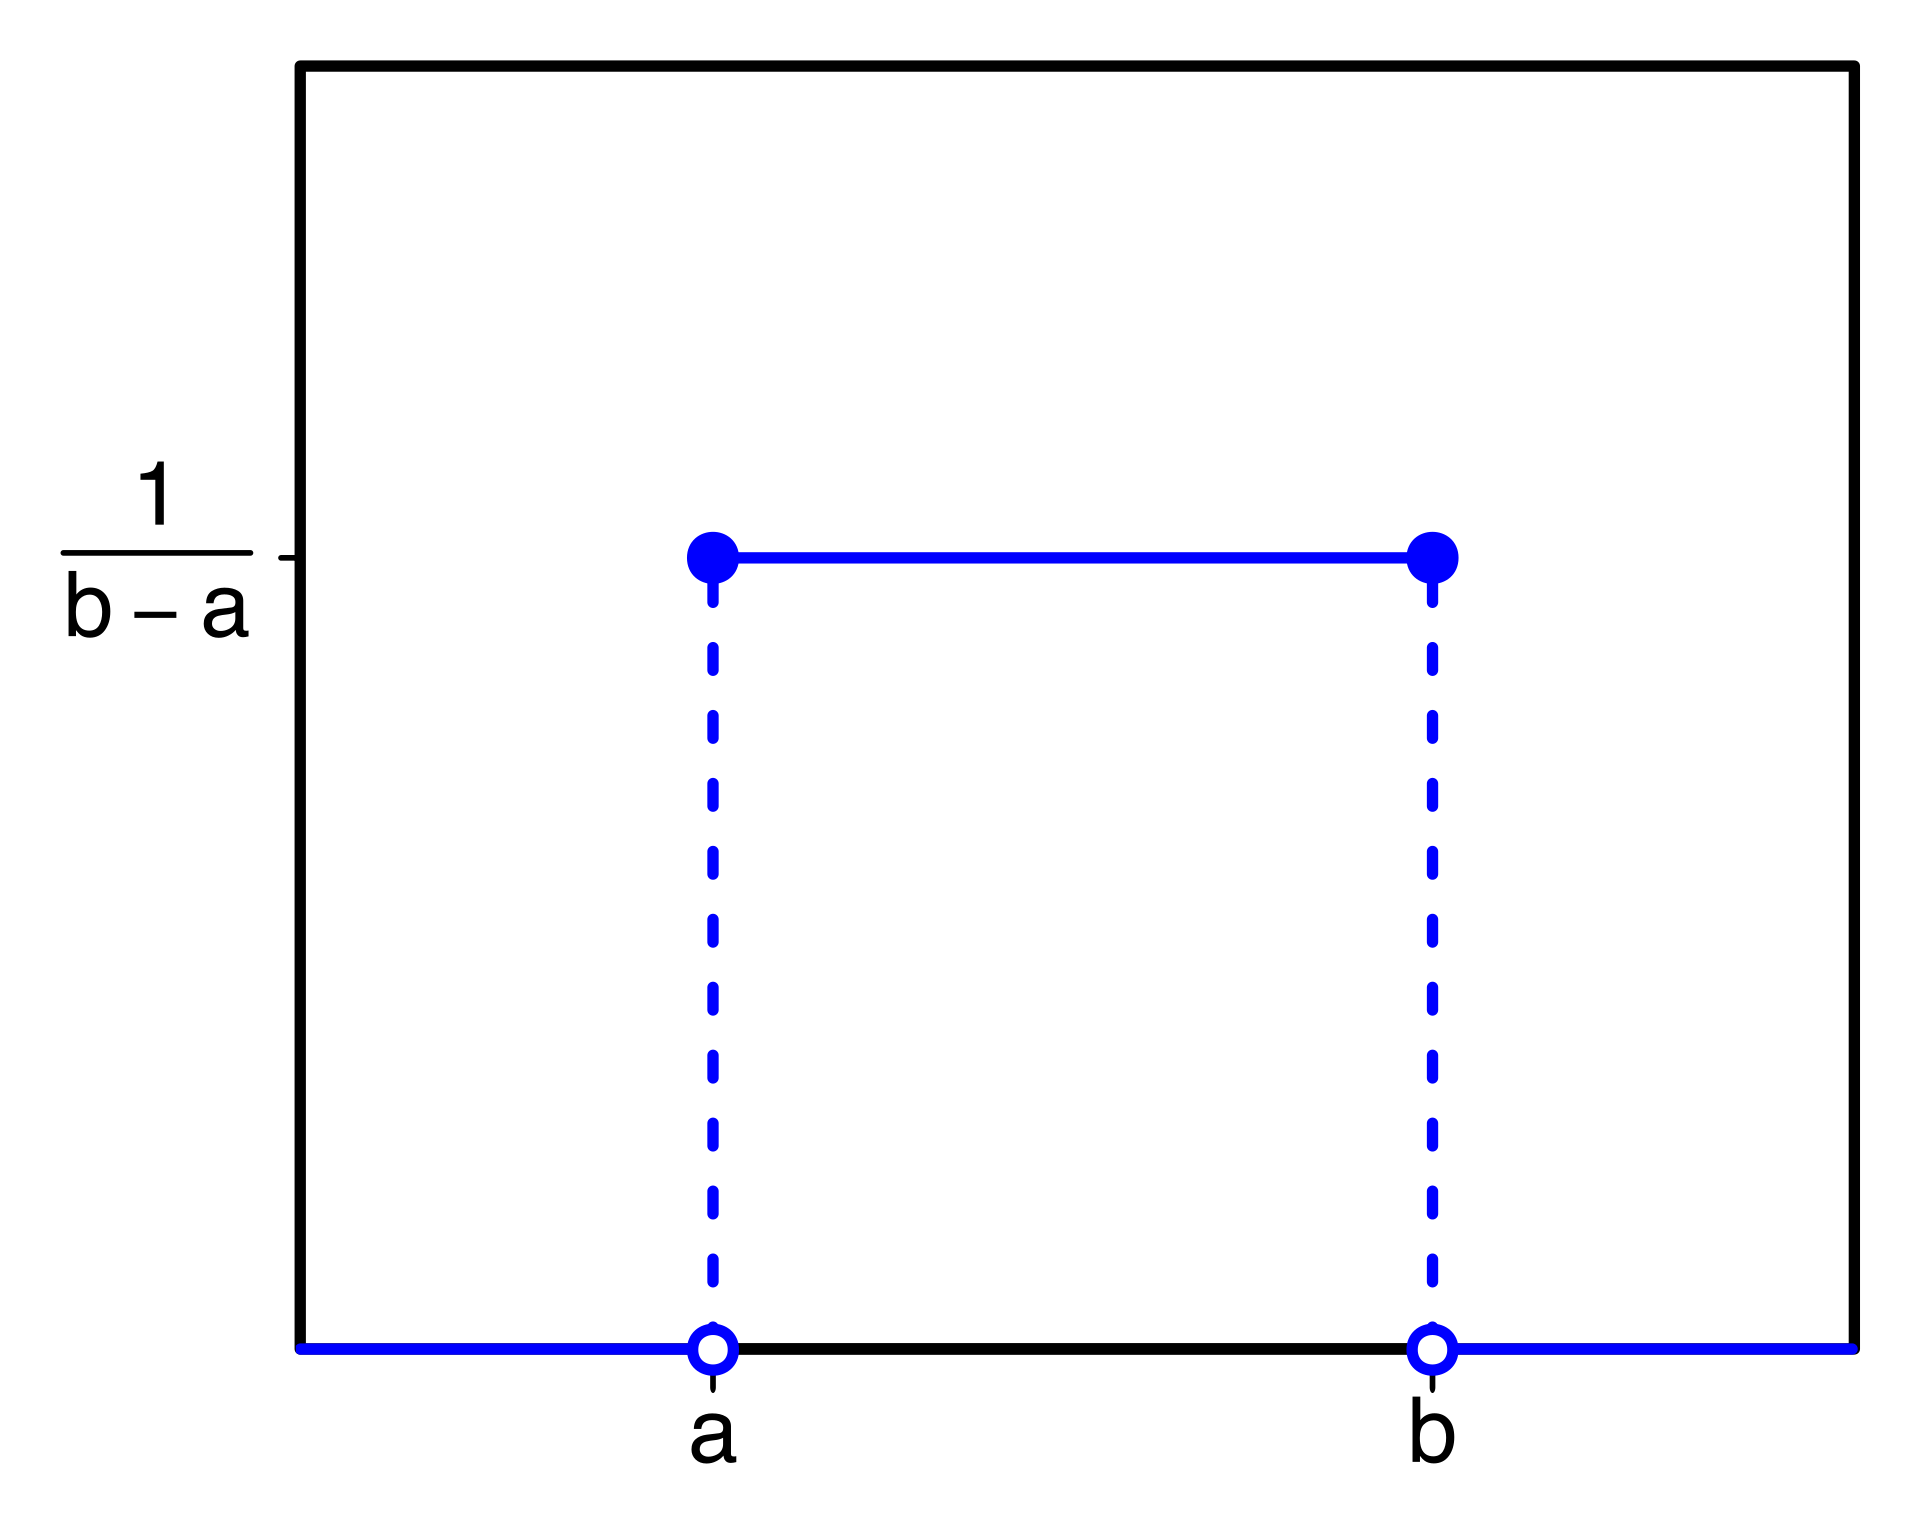
\includegraphics[width=0.5\linewidth]{assets/uni_f.png}
    \caption{Функция плотности равномерного распределения}
    \label{fig:}
    \end{center}
\end{figure}

\begin{figure}[H]
    \begin{center}
    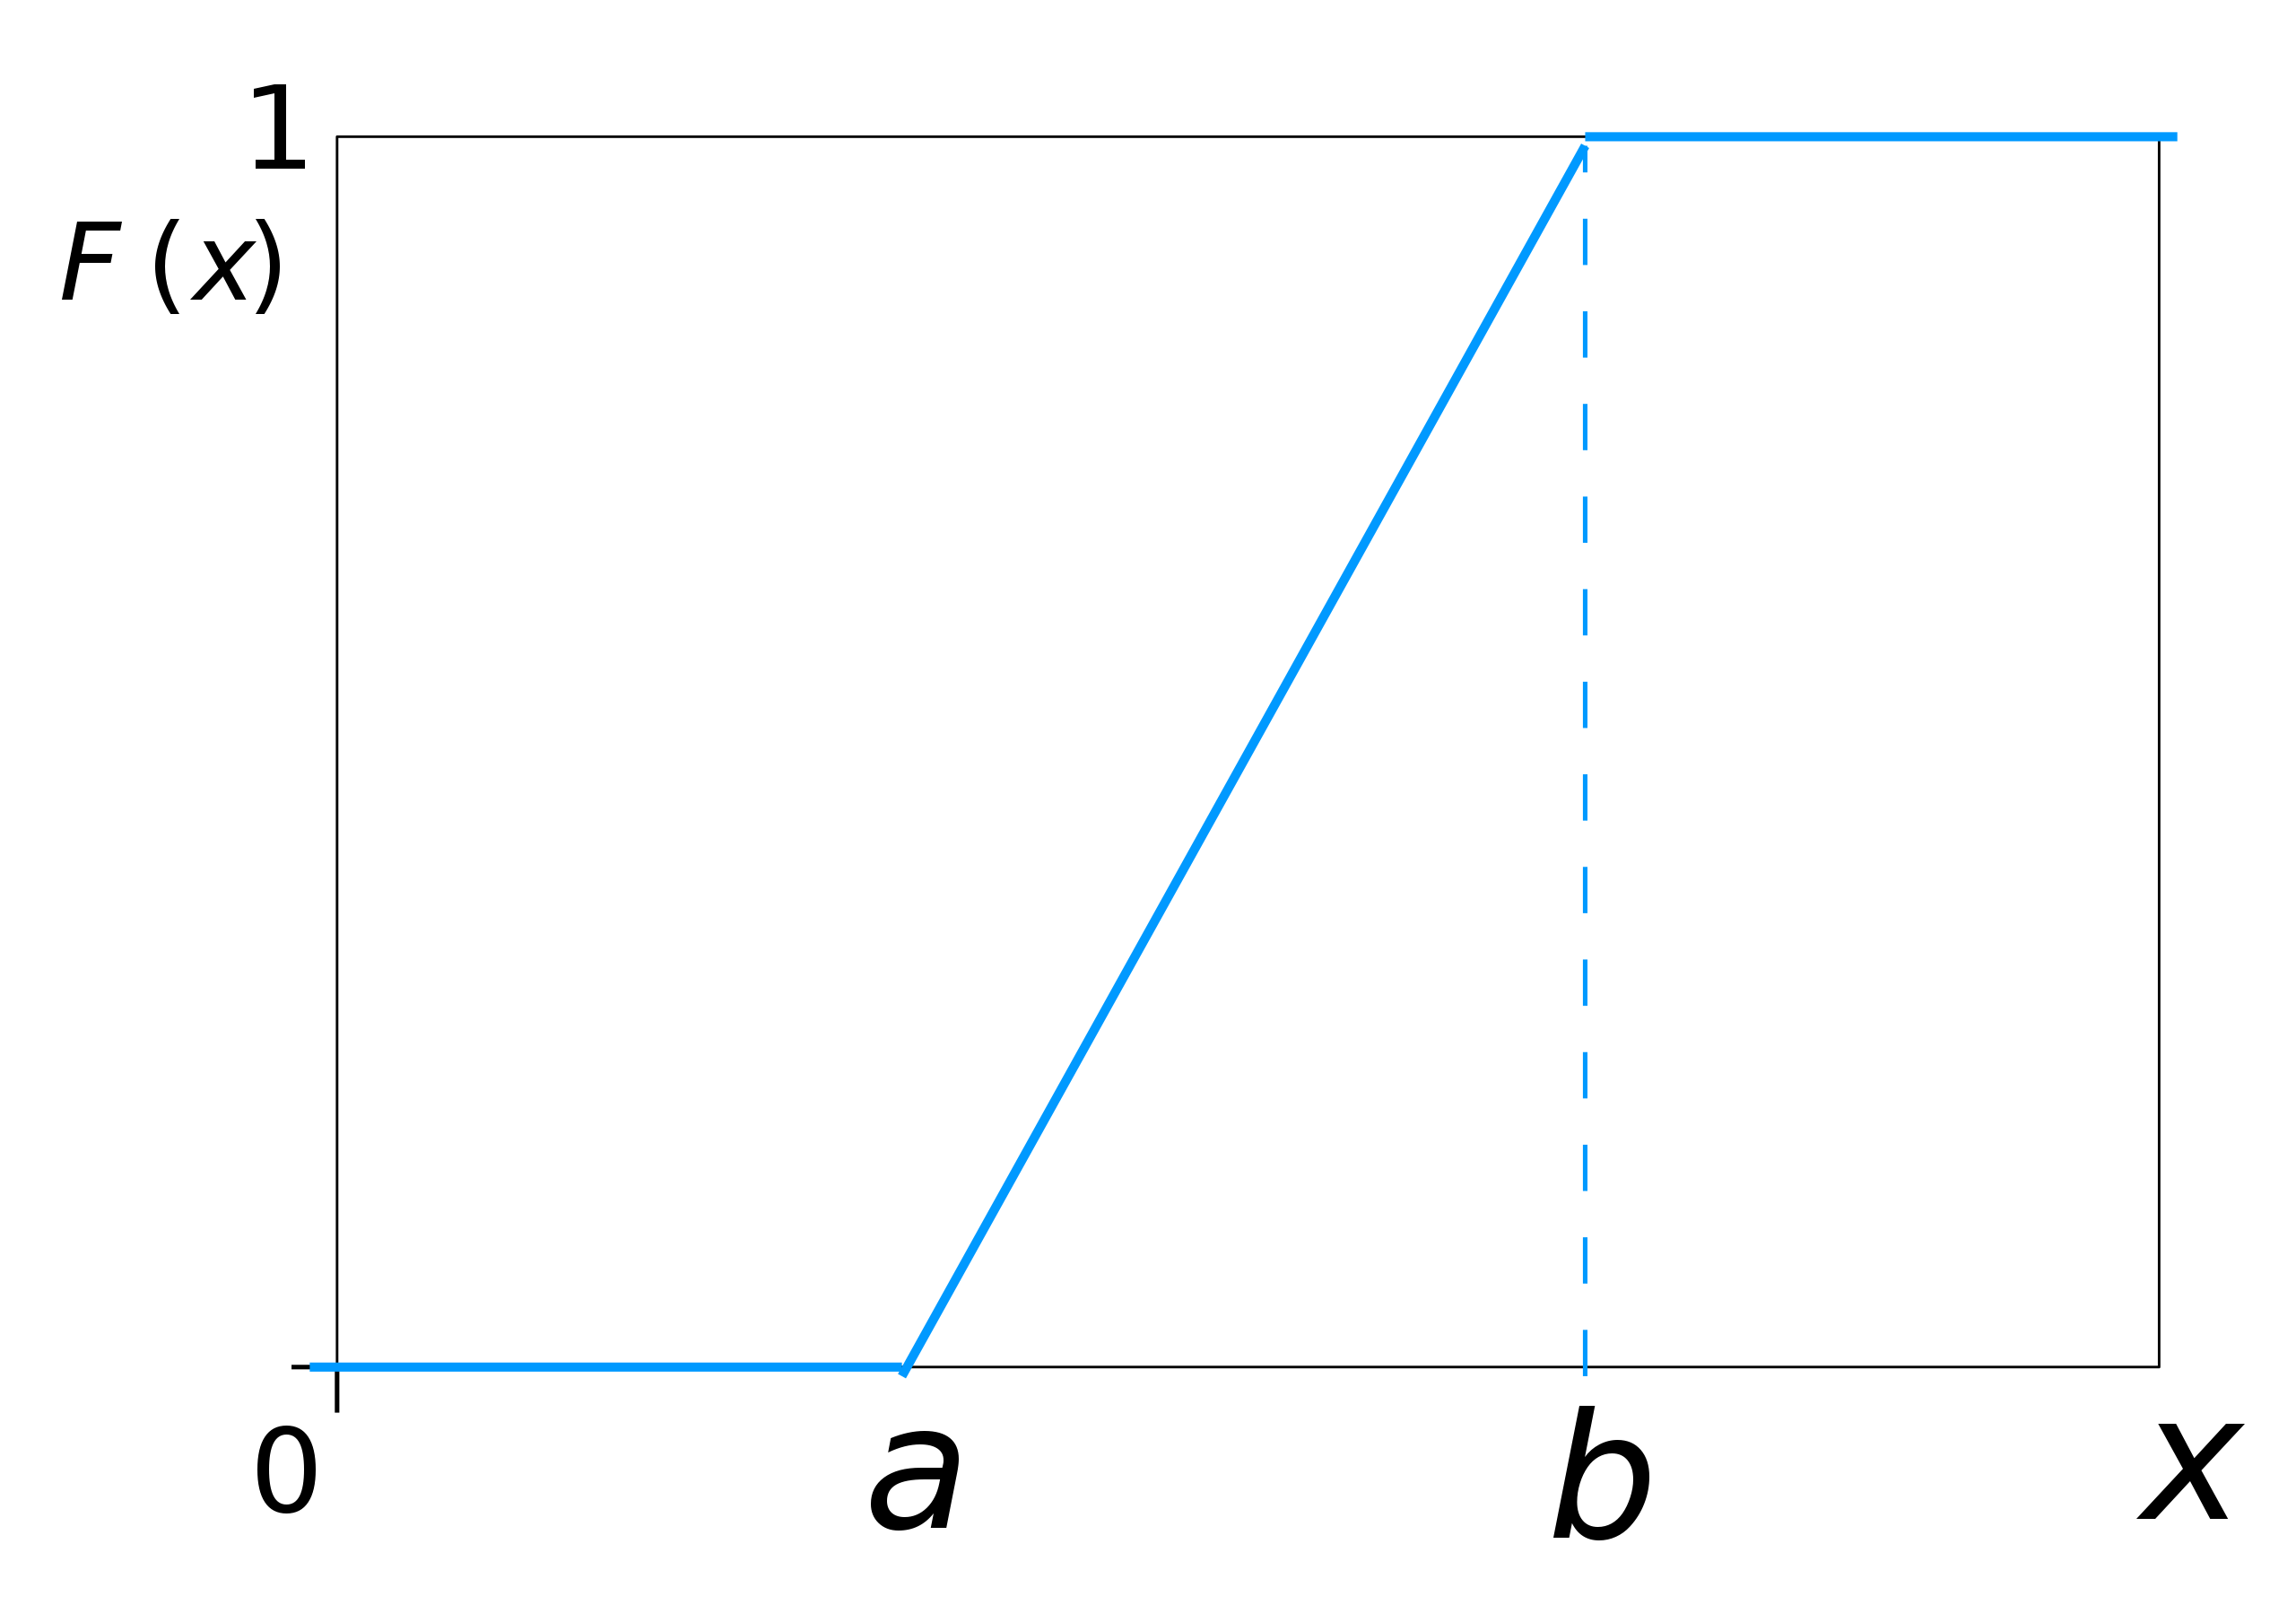
\includegraphics[width=0.5\linewidth]{assets/uni_Fx.png}
    \caption{Функция распределения равномерного распределения}
    \label{fig:}
    \end{center}
\end{figure}

\subsection{Распределение Эрланга}

Распределение Эрланга является непрерывным распределением, ограниченным снизу. Оно представляет собой особый случай Гамма распределения, где параметр $k$ может принимать только положительные целые значения.

Функция распределения:

\begin{equation*}
F_X(x) = 1 - \sum_{i=0}^{k-1}  \frac{1}{i!} e^{-\lambda x} (\lambda x)^n
\end{equation*}
    
Плотность распределения:

\begin{equation*}
f_X(x) = \frac{\lambda^k x^{k-1} e^{-\lambda x} } {(k-1)!}
\end{equation*}

\begin{figure}[H]
    \begin{center}
    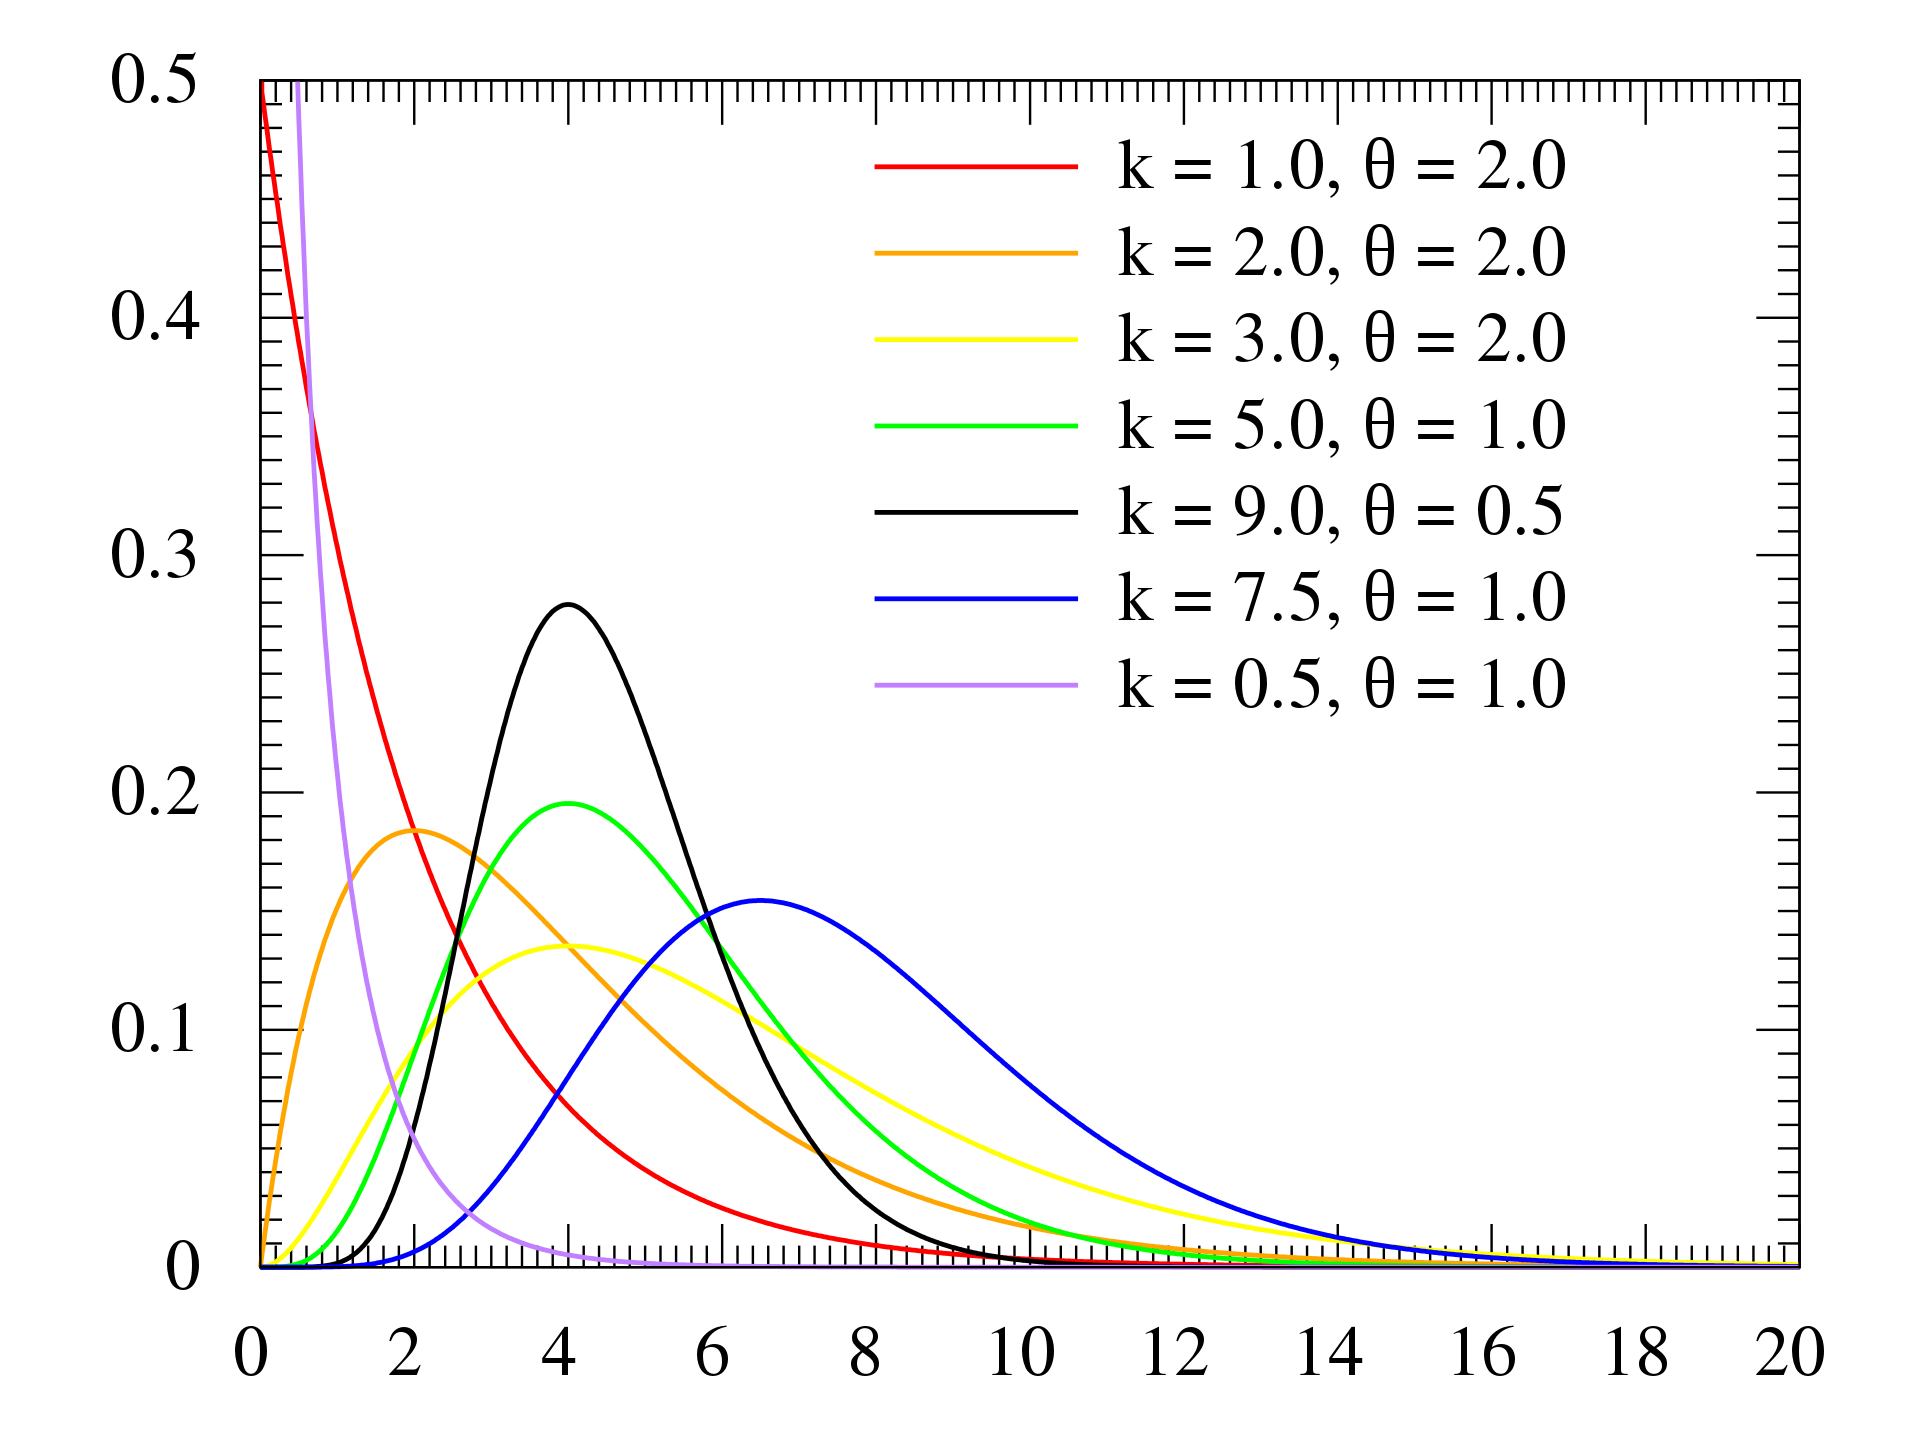
\includegraphics[width=0.5\linewidth]{assets/erlang_f.png}
    \caption{Функция плотности распределения Эрланга}
    \label{fig:}
    \end{center}
\end{figure}

\begin{figure}[H]
    \begin{center}
    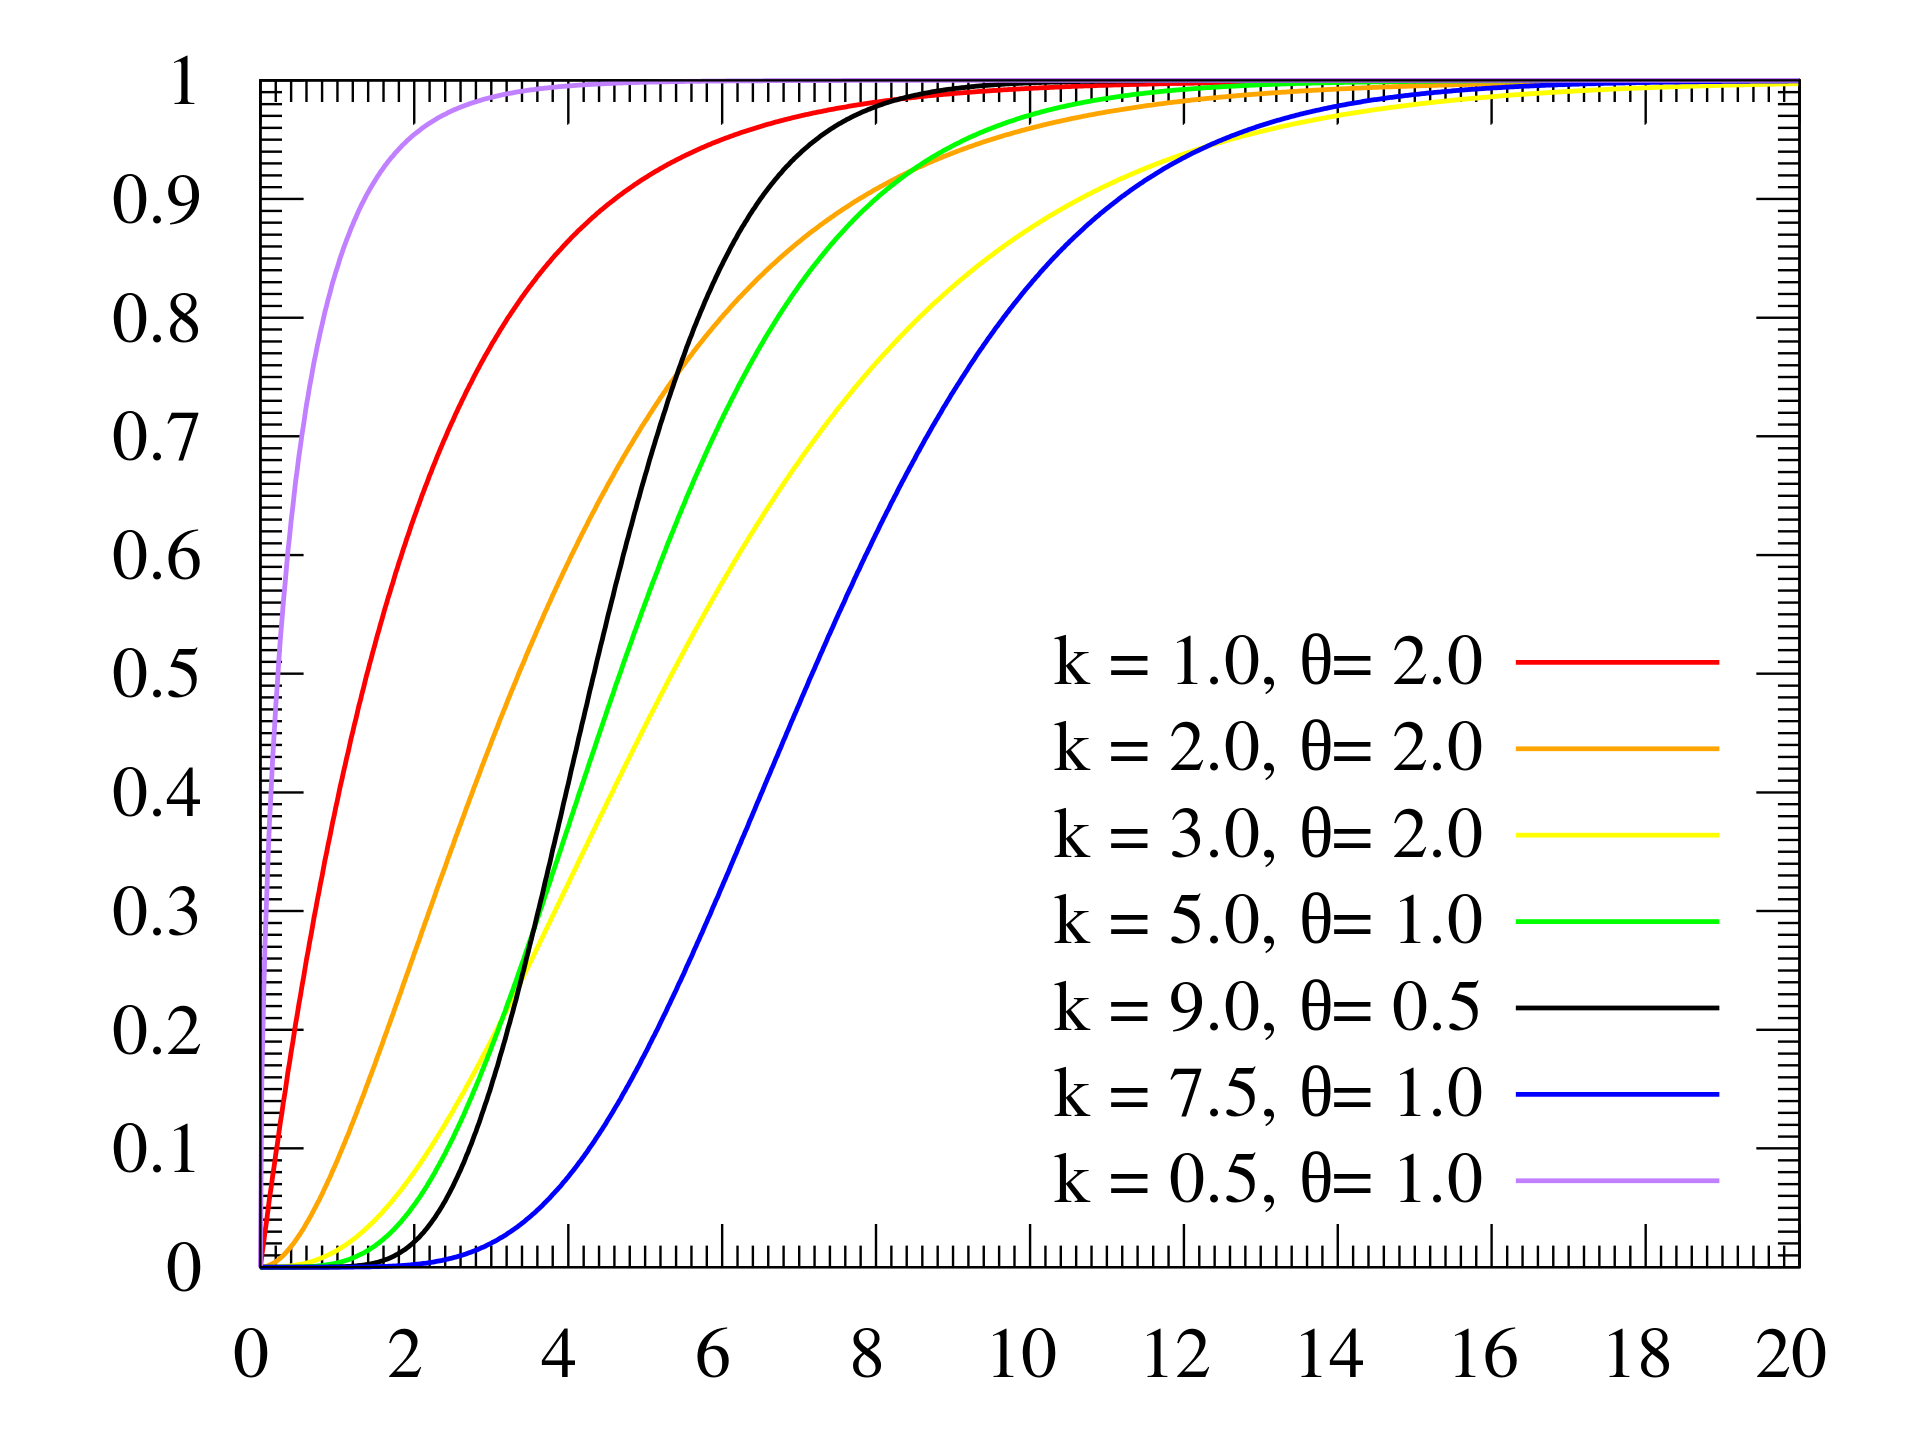
\includegraphics[width=0.5\linewidth]{assets/erlang_Fx.png}
    \caption{Функция распределения распределения Эрланга}
    \label{fig:}
    \end{center}
\end{figure}

\section{GPSS}

Система GPSS World~---~мощная универсальная среда моделирования как дискретных, так и непрерывных процессов, предназначенная для профессионального моделирования самых разнообразных процессов и систем. Эта система явилась следующим шагом развития системы GPSS/PC (1984 год), ориентированной на DOS. Обе системы разработаны специалистами фирмы Minuteman Software (основана в 1982 году) под руководством Спрингера Кокса. Сначала система GPSS World появилась в 1994 году с ориентацией на OS/2 фирмы IBM, и только в 2000 году она была реализована под ОС Windows фирмы Microsoft.

С помощью этой системы, например, можно эффективно моделировать как производственные, так и непроизводственные процессы: функционирование торговых и увеселительных заведений, портов, уличное движение, проведение военных действий, работу редакций, учреждений и сети Internet, различных систем массового обслуживания и~т.~д. Система имеет большой набор команд для управления процессом моделирования, которые можно как использовать в интерактивном режиме, так и включать в модель. Обеспечена возможность проведения экспериментов, сгенерированных системой, пользовательских и оптимизационных. В системе GPSSW реализована процедура визуализации процесса функционирования модели с использованием методов мультипликации.

Система GPSSW имеет новый высокоскоростной транслятор, работающий в сотни раз быстрее его предшественников. Для быстрого исправления ошибок используется полноэкранный текстовый редактор.

